\begin{figure}[H]
    \centering
    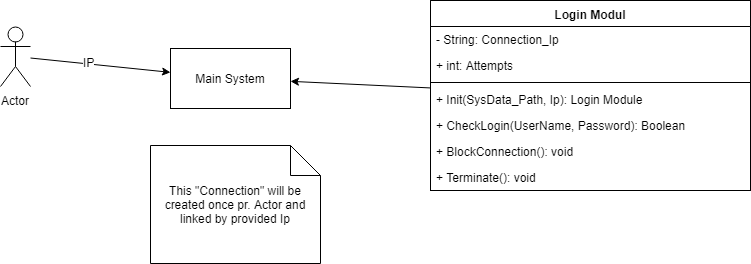
\includegraphics[width=1\linewidth, height=6cm]{Struktureret_System_Udvikling/Workshop_1/Assets/ClassDiagram.png}
    \caption{Class Diagram}
    \label{fig:my_label}
\end{figure}

\noindent
\\Som ses på ovenstående diagram har gruppen valgt en af de førnævnte use cases, til en nærmere beskrivelse. i dette tilfælde er der valgt use case \#2. Login.
Denne indeholder 2 moduler, navngivet CheckLogin og BlockConnection, foruden de 2 fastsatte, henholdvis constructor og destroyer. Idéen bag denne implementation er at modulet initieres for hver forsøgende forbindelse, identificeret via den forbindende kontakts ip-addresse. Foruden denne ip initieres modulet også med en given path, til en system fil indeholdende systemets login kriterier, og en liste over blokerede ip'er.
Her efter kan CheckLogin anvendes til at checke om et set loginoplysninger fra den forbindende bruger er sand, da denne returnere sand ved korrekte loginoplysninger. Samtidigt kan denne også bruges til at fange mulige angreb da hvis de angivne oplysninger ikke er sande, vil modulets interne tæller "Attempts" tælle op, og derfor vil denne kunne anvendes til at identificere eventuelle angreb.
Ved identifikation af et sådant angreb vil BlockConnection herefter kunne tilføje modulets initierede forbindelses ip til listen i systemfilerne over blokerede forbindelser.
Og tilsidst kan modulet Terminieres.

\noindent
\\For Usecase #2. Login\\
Ville Overstående Modul skulle anvendes i følgende sammenhæng:\\
\noindent
0. Check if connecting IP is part off blocklist, from SysData
\\1. Init()\\
- With path to lib providing sys kalibrated data\\
- And the connection IP\\
- Init returns error if provided connection Ip is part of Block List
\\2. CheckLogin()\\
- With User provided login credentials\\
3.1 If CheckLogin returns False:\\
- If Attempts for current connection Module more than 5 BlockConnection()\\
3.2 If CheckLogin returns True:\\
- Send user to administration page (Login is done) \\
4. Terminate()